% Materialer og metoder 2/5
%I dette kapitlet skal du skrive om hvordan du har gått frem metodisk, og vise hvordan valg av design og metode egner seg til å svare på problemstillingen din.

%Kapitlet må kunne gi svar på disse spørsmålene:

%Hvordan samlet du inn datamaterialet?
%Hvordan behandlet du dataene du samlet inn?
%Hvorfor valgte du disse metodene?
%Hva er styrkene og svakehetene ved disse metodene?
%Du skal også si noe om hvorfor du har gjort din undersøkelse på den måten du gjorde – og da peke på styrker og svakheter. I tillegg skal du drøfte etiske aspekter ved prosjektet. På den måten viser du at du har kommet frem til resultatene på en pålitelig og troverdig måte, men også at du er reflektert og kritisk overfor arbeidet du har gjort.

%Husk også at du her, slik som i teorikapitlet, bare skal skrive om det metodiske som er relevant for din studie.
\section{Metode}

\begin{figure}[h!]
\begin{center} 
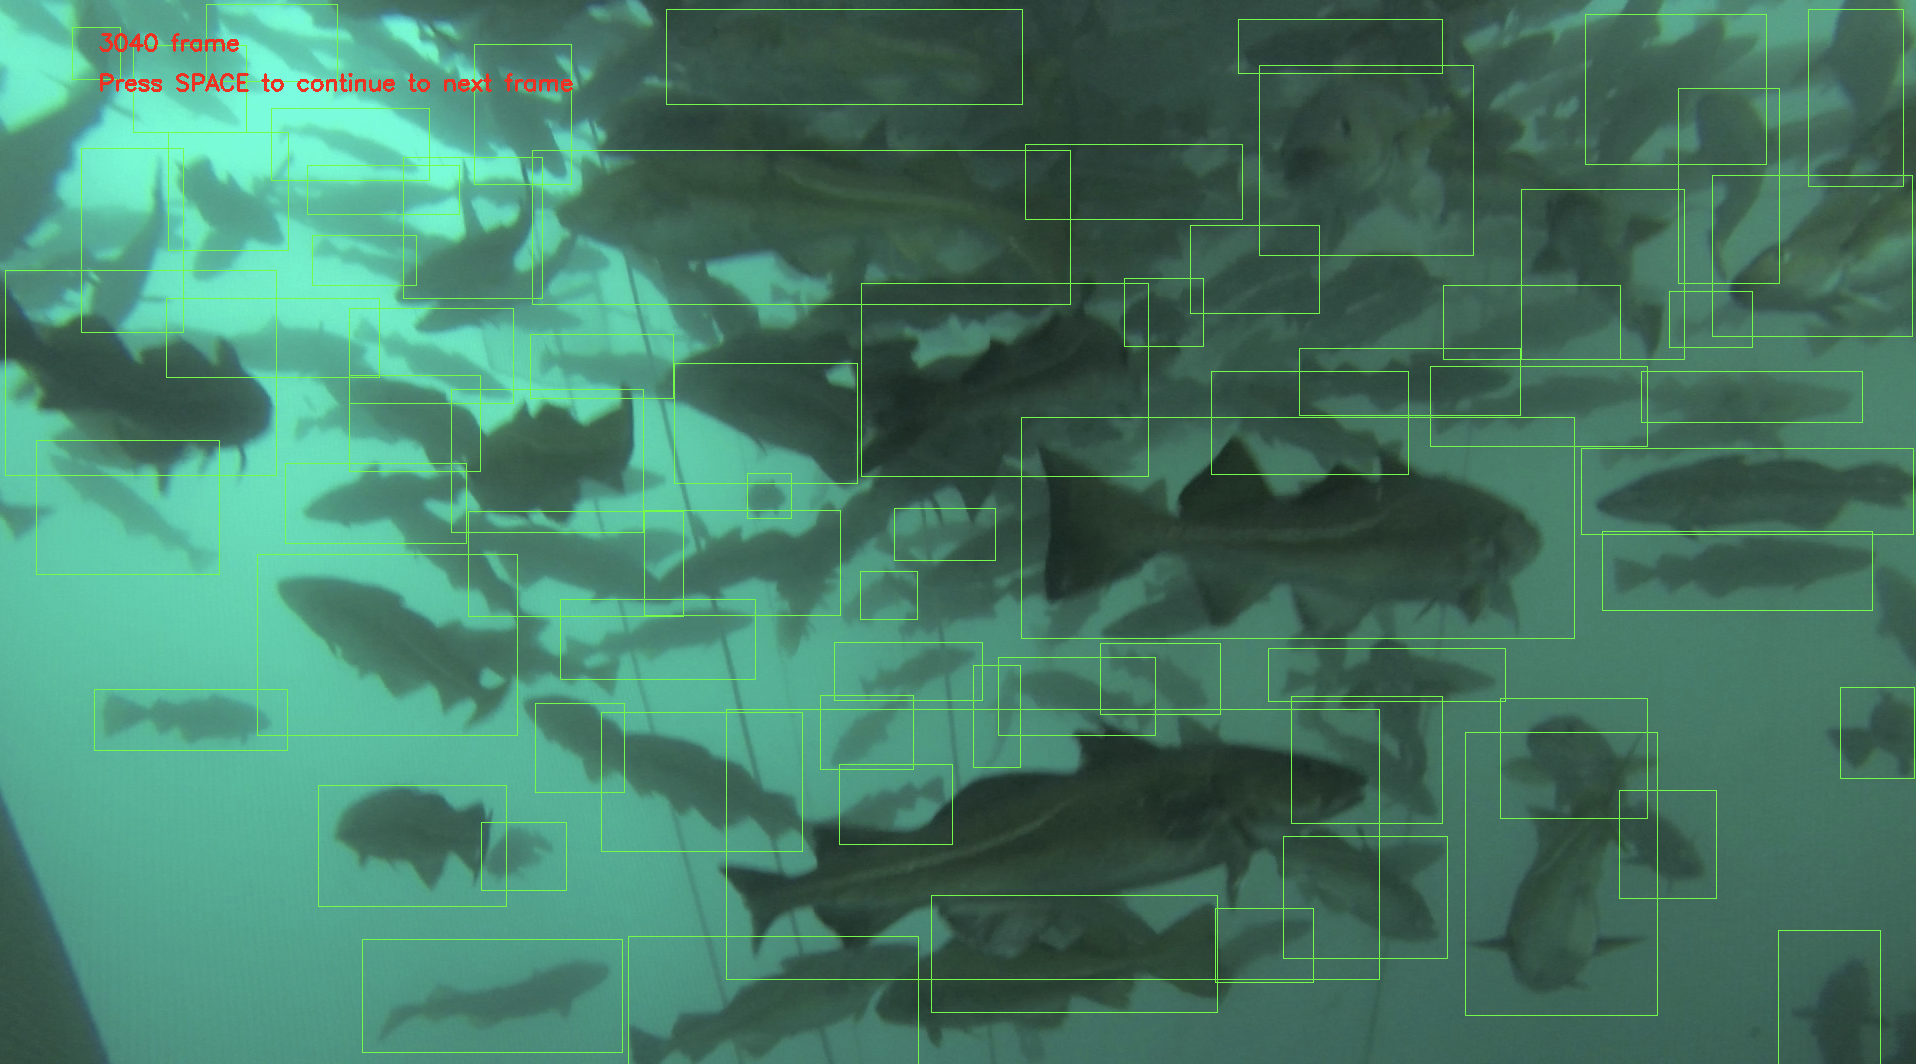
\includegraphics[scale=0.35]{figures/dataset_tool_2}
\caption{\small \sl Figuren viser et dataprogram som ble utviklet for å lage label data basert på opptakene fra Nofima. Dataprogrammet laster inn hvert femtiende bilde fra en video av en lagringsmerd av torsk. Denne videoen er 7 minutter lang. På figuren vises bilde nummer 3040. En modell som kan detektere objekter krever å bli trent på bilder av det den skal kjenne igjen, bilder med label data. Label data består av klassenummer, og `xmin', `ymin', `xmax', og `ymax' posisjoner, som skaper et rektangel rundt objektene som finnes i bildet, for hvert objekt som finnes i treningsdataen. Med dette dataprogrammet så er å lage slik informasjon fra et bilde enkelt, brukeren trenger kun å lage et rektangel rundt hver torsk. Klassenummeret for torsk, her 0, og posisjonene av rektangelet, `xmin', `ymin', `xmax', og `ymax', kjent som objektets ground truth bounding box, lagres til en tekstfil. Rådataen, bilde uten rektanglene eller den røde teksten som er øverst i venstre hjørne, lagres også automatisk til en mappe. \label{fig:dataset_tool}} 
\end{center} 
\end{figure} 

%Dette kapitlet er obligatorisk for alle forsøksoppgaver. Det bør innledes med et flytskjema/oversikt og en beskrivelse som letter leserens forståelse av hva som er gjort. Dette gjelder både for rene analyseoppgaver og for produktutviklingsoppgaver. 

%Beskrivelsen av materialer og metoder skal være tilstrekkelig detaljert slik at andre kan vurdere arbeidet og om ønskelig gjenta forsøkene. Samtidig må man unngå å fylle opp rapporten med unødige detaljer. Dersom det er brukt en velkjent metode, er det nok å bruke metodens offisielle navn og henvise til offisiell kilde. Hvis det var nødvendig med modifikasjoner eller andre tilpasninger i forhold til metoden, må dette beskrives. Eventuell teori om metoden, hører hjemme i teoridelen. Beskriv det dere har gjort og ikke det dere skulle ha gjort. 

%Hensikten med kapitlet Materialer og metoder er at andre skal kunne utføre det samme arbeidet på samme måte. Da må alle nødvendige opplysninger være med.

Trening av kunstige nevrale nettverk gjøres i seks steg. Det ble trent opp to modeller, en RetinaNet modell og en YOLOv4 modell. RetinaNet hadde forhåndstrente vekter fra en modell trent på COCO datasettet til Microsoft, og YOLOv4 hadde fohåndstrente vekter fra en modell trent på ImageNet datasettet, modellene ble ikke trent fra scratch. %You should design a model which achieves 85 \% validation accuracy on the given dataset.

Microsoft Azure plattformen ble anvendt til å trene modellene. Microsoft tilbyr Nvidia Titan GPU-er i skyen. Å anvende GPU-er når en trener kunstige nevrale nettverk gjør at treningen tar mindre tid.

Det tok ca. 2 dager å trene YOLOv4 modellen på nettskyen Azure med maskinstørrelsen Standard NC6 Promo (6 vcpu-er, 56 GiB dataminne). Trening av RetinaNet tok mye mindre tid, men inferens av RetinaNet tok over seks timer for 7 minutter video. YOLOv4 kan gjøre inferens på noen millisekunder per bilde, der RetinaNet bruker titals sekunder selv på kraftig maskinvare.% Se figur retinanet vs YOLOv4 resultater

Kildekoden for prosjektet kan lastes ned fra: \\ \url{https://github.com/alanhaugen/TMAT3004-Bacheloroppgave}.

\subsection{Å forstå problemet}

Før en begynner så er det viktig å være sikker på at man forstår problemet en skal løse. I denne oppgaven så skulle mengden av to fisk, torsk og sei, telles med maskinsyn. Det er to klasser. For å løse denne oppgaven kreves bilder av hver fisk med korrekt label-data og et rimelig stort nettverk som kan forstå og trenes på bilder.

Objektdeteksjon handler om to ting. Områder av bilde som kan inneholde en klasse må genereres, og så må disse delene av et bilde klassifiseres basert på det visuelle innholdet i bildeområdet, et bildeområde kalles for en patch innenfor maskinsyn. Områdene der det kan være objekter kalles for ankre. Med andre ord, målet for modellen er å se på en del av et bilde og finne ut hvilket objekt som finnes i dette området. Nettverket kan kun finne de objektene som den har blitt trent til å gjenkjenne.

\subsection{Få tak i data}

Det neste steget var å få tak i data. Datasettet som ble laget for dette prosjektet bestod av bilder fra en lagringsmerd av torsk, og bilder av sei fra Havbruksstasjonen i Tromsø. Se figur \ref{fig:data} og \ref{fig:nofima}. Opptakene av fiskene ble laget av Nofima og ble omgjort til bilder. Label data lagt inn manuelt. Se figur \ref{fig:dataset_tool}. Dataen av torsk var fargebilder, så de bestod av tre kanaler, og hadde størrelsen 1920 $\times$ 1080. Bildene av sei var gråtoner, kun en kanal, og hadde størrelsen 640 $\times$ 480. %You need to achieve 85 \% accuracy for validation data to successfully complete this assignment. Check it out here.

\begin{figure}[h!]
\begin{center} 
\includegraphics[scale=0.05,angle=-90,origin=c]{figures/camera_1}
\includegraphics[scale=0.05,angle=-90,origin=c]{figures/camera_2}
\includegraphics[scale=0.05]{figures/camera_3}
\caption{\small \sl Figuren viser kamerautstyret som ble anvendt til å lage seidataen. Nofima anskaffet et undervannskamera av typen Steinsvik Orbit-3300 som styres via et MB-3000 kontrollpanel. \label{fig:nofima}} 
\end{center} 
\end{figure} 

Datasettet bestod av 208 bilder av torsk, med til sammen 4582 instanser av torsk i bildene. Det var 604 bilder av sei med 5525 instanser av fisken i bildene. Bildene av torsk og sei ble satt i hver sin mappe. De ble splittet etter forholdet 80/20, 80 \% av dataen var for trening, og 20 \% for validering.

\subsubsection{Utforsk og forstå dataen}

Det er viktig å se på dataen før en begynner å trene et nettverk. Det er viktig å se etter bias i bildene. Det er lurt å gå igjennom hvert eneste bilde, og se om det er noe en kan lære. Torsk og sei bildene kunne bli augmented, de kunne blant annet bli snudd horisontalt. Det gir dobbelt så mye treningsdata. Vær obs på at ikke alle treningssett tillater dette, for eksempel et datasett med lego.

Det var to klasser i datasettet, torsk og sei. Se figur \ref{fig:tree} og tabell \ref{tab:classes}.

\begin{figure}[h!]
\Tree[.data [.labels ] [.train [.atlantic\_cod ]
               [.saithe ]]
          [.validation [.atlantic\_cod ]
                [.saithe ]]]
\caption{\small \sl Figuren viser et tre av mappestrukturen til datasettet. \label{fig:tree}} 
\end{figure} 

\begin{table}[h!]
\bigskip
\centering
\caption{Klassenavn og navneenkoding for datasettet}
\label{tab:classes} 
\begin{tabular}[t]{lcc}
\toprule
Klassekode & Klassenavn    & Norsk klassenavn \\
\midrule
0          & atlantic\_cod & torsk            \\
1          & saithe        & sei         \\
\bottomrule	
\end{tabular}
\end{table}

`Labels` mappen inneholdt bounding box data for bildene. Det var en eller flere linjer per `.txt` fil. Hver linje representerer en bounding box. Representasjonen er i `xmin', `ymin', `xmax', og `ymax' formatet. Se tabell \ref{tab:bbox}.

Filene som ble brukt til trening og validering ble definert i data\/fish\_train.txt og data\/fish\_test.txt. Se tabell \ref{tab:fish}.

\begin{table}[b]
\bigskip
\centering
\caption{Label data for bilde data\/train\/atlantic\_cod\/fish\_9440.png, lagt i fil data\/labels\/fish\_9440.txt}
\label{tab:bbox} 
\begin{tabular}[t]{lcccc}
\toprule
Klassekode    & xmin      & ymin    & xmax     & ymax \\
\midrule
0 & 238 & 643 & 582 & 882 \\
0 & 80   & 858 & 368 & 1071 \\
\bottomrule	
\end{tabular}
\end{table}

\begin{table}[b]
\bigskip
\centering
\caption{Eksempel på filnavn i data\/fish\_train.txt og data\/fish\_test.txt}
\label{tab:fish} 
\begin{tabular}[t]{c}
\toprule
Filnavn i fish\_test.txt \\
\midrule
validation/atlantic\_cod/fish\_590.png \\
validation/atlantic\_cod/fish\_640.png \\
\vdots \\
\bottomrule	
\end{tabular}
\end{table}

\subsection{Gjør klar dataen}

Da dataen hadde blitt organisert, og label data nøye konstruert, så ble nettverkene konfigurert og treningen ble satt i gang. Dataen ble matet inn i treningsprogrammet, inn i deep learning rammeverkene.

Det ble trent opp to nettverk. Den ene, RetinaNet, er en del av detectron2 fra Facebook. Den ble trent og konfigurert med PyTorch. Den andre modellen var YOLOv4, den trenes med deep learning rammeverket darknet. Konfigurasjon gjøres ved å endre på tekstfiler og kommandolinjeparameterene til rammeverket.

\subsubsection{Dataaugmentering}

Dataen må først normaliseres på en standard måte, for eksempel ved å subtrahere gjennomsnittet over dataen, for så å skalere alle bildene slik at de får samme størrelse. Det er også mulig å gjøre flere andre endringer. Støy kan legges til bildene, samt å snu dem horisontalt eller vertikalt for å skape nye bilder å trene nettverket på.

Det ble ikke gjort endringer på standardmåten detectron2 og darknet gjør dataaugmentering.

\subsubsection{YOLOv4 label data og bildeformat}

YOLOv4 har et annet label-format sammenlignet med RetinaNet, dessuten krever den bilder i jpeg formatet, med filudvidelsen .jpg. Label-dataen legges sammen med bildene. Konvertering fra RetinaNet sitt format til YOLOv4 ble gjort med et awk-skript. Formatet til YOLOv4 er:

\begin{verbatim}
[klassenavn] [objekt midtpunkt i X] [objekt midtpunkt i Y]
	[objekt vidde i X] [objekt høyde i Y]
\end{verbatim}

Et nyttig verktøy til å konvertere bilder er John Cristy sin Image Magick. Her er hvordan bildene ble konvertert fra Adobe sitt png format til jpeg:

\begin{verbatim}
mogrify -format jpg *.png
\end{verbatim}

\subsection{Tren nettverket på et lite utvalg av dataen som en test før en trener et fullt nettverk}

Nettverket ble først trent opp på et utvalg av treningsdataen, for å teste nettverket. 208 bilder med 4582 instanser av torsk ble grunnlaget for de første RetinaNet og YOLOv4 modellene. Dette steget gjøres som en sanity check før en begynner på trening som kan ta mange timer.

RetinaNet modellen ble trent med en learning rate på 0,001 over 500 iterasjoner. Modellen brukte vekter fra COCO, den ble lastet ned fra the model zoo, den heter COCO-Detection\/retinanet\_R\_50\_FPN\_3x.yam. RetinaNet sin score threshold ble satt til 0,5. Batch size var 4.

\subsubsection{RetinaNet konfigurasjon og trening}

RetinaNet er implementert i detectron2, som bruker deep learning rammeverket PyTorch. Grensesnittet er programmeringsspråket Python. Detectron2 er utgitt under en Apache 2.0 lisens, det vil si at den kan brukes til hva enn en vil på en hvilken som helst måte, gratis, så lenge man aksepterer at facebook ikke blir ansvarlig for arbeidet som gjøres, og så lenge man ikke krediterer arbeidet en gjør til facebook \cite{The Apache Software Foundation 2004}. Detectron2 installeringsinstrukser er tilgjengelig her: \url{https://detectron2.readthedocs.io/}

Først må bibliotekene lastes inn. Se python koden under.

\begin{lstlisting}[language=Python, caption=Her lastes bibliotekene inn i train.py for detectron2]
import torch
import detectron2
#import onnx
#from detectron2 import export
from detectron2.utils.logger import setup_logger
setup_logger()

# import some common libraries
import numpy as np
import cv2
import random
import os
import matplotlib.pyplot as plt

# model_zoo has a lots of pre-trained model
from detectron2 import model_zoo


# DefaultTrainer is a class for training object detector
from detectron2.engine import DefaultTrainer
# DefaultPredictor is class for inference
from detectron2.engine import DefaultPredictor

# detectron2 has its configuration format
from detectron2.config import get_cfg
# detectron2 has implemented Visualizer of object detection
from detectron2.utils.visualizer import Visualizer

# from DatasetCatalog, detectron2 gets dataset and from MetadatCatalog it
# gets metadata of the dataset
from detectron2.data import DatasetCatalog, MetadataCatalog

# BoxMode support bounding boxes in different format
from detectron2.structures import BoxMode

# COCOEvaluator based on COCO evaluation metric, inference_on_dataset is used for
# evaluation for a given metric
from detectron2.evaluation import COCOEvaluator, inference_on_dataset

# build_detection_test_loader, used to create test loader for evaluation
from detectron2.data import build_detection_test_loader

\end{lstlisting}

Konfigurasjonen defineres i neste kodesnutt.

%\begin{lstlisting}[language=Python, caption=Treningen og testingen, samt operativssystemet konfigureres]
\begin{lstlisting}[language=Python, caption=Konfigurasjon i train.py]
data_root = 'data'
train_txt = 'fish_train.txt'
test_txt  = 'fish_test.txt'

train_data_name = 'fish_train'
test_data_name  = 'fish_test'

thing_classes = ['atlantic_cod', 'saithe']

output_dir = 'outputs'

def count_lines(fname):
    with open(fname) as f:
        for i, l in enumerate(f):
            pass
    return i + 1

train_img_count = count_lines(os.path.join(data_root, train_txt))

# Register train and test data
# dataset can be registered only once with one name

# register train data
DatasetCatalog.register(name=train_data_name,
                        func=lambda: get_fish_dicts(data_root, train_txt))
train_metadata = MetadataCatalog.get(train_data_name).set(thing_classes=thing_classes)

# register test data
DatasetCatalog.register(name=test_data_name,
                        func=lambda: get_fish_dicts(data_root, test_txt))
test_metadata = MetadataCatalog.get(test_data_name).set(thing_classes=thing_classes)

# default configuration
cfg = get_cfg()

# update configuration with RetinaNet configuration
cfg.merge_from_file(model_zoo.get_config_file("COCO-Detection/retinanet_R_50_FPN_3x.yaml"))
cfg.MODEL.ROI_HEADS.SCORE_THRESH_TEST = 0.5

# We have registered the train and test data set with name fish_train and fish_test.
# Let's replace the detectron2 default train dataset with our train dataset.
cfg.DATASETS.TRAIN = (train_data_name,)

# No metric implemented for the test dataset, we will have to update
# cfg.DATASET.TEST with empty tuple
cfg.DATASETS.TEST = ()

# data loader configuration
cfg.DATALOADER.NUM_WORKERS = 4

# Update model URL in detectron2 config file
cfg.MODEL.WEIGHTS = model_zoo.get_checkpoint_url("COCO-Detection/retinanet_R_50_FPN_3x.yaml")
model_final_f10217.pkl"
\end{lstlisting}

Konfigurasjonen av batch size, data path og learning rate er de viktigste variablene, det er det neste som settes her. 

\begin{lstlisting}[language=Python, caption=Solver konfigurasjon i train.py]
# batch size
cfg.SOLVER.IMS_PER_BATCH = 4

# choose a good learning rate
cfg.SOLVER.BASE_LR = 0.001

# We need to specify the number of iteration for training in
# detectron2, not the number of epochs.
# lets convert number of epoch to number or iteration (max iteration)

epoch = 1000
max_iter = int(epoch * train_img_count / cfg.SOLVER.IMS_PER_BATCH)
max_iter = 500

cfg.SOLVER.MAX_ITER = max_iter

# number of output class
cfg.MODEL.RETINANET.NUM_CLASSES = len(thing_classes)

# update create ouptput directory
cfg.OUTPUT_DIR = output_dir
os.makedirs(cfg.OUTPUT_DIR, exist_ok=True)

\end{lstlisting}

Neste kodesnutt er trening, resultatene finnes på tensorboard: \\
\url{https://tensorboard.dev/experiment/aZzjBUzKTAy19KPsDZPJ2g}

\begin{lstlisting}[language=Python, caption=Treningskode i train.py]
# Create a trainer instance with the configuration.
trainer = DefaultTrainer(cfg) 

# if rseume=False, because we don't have trained model yet. It will
# download model from model url and load it
trainer.resume_or_load(resume=False)

# start training
trainer.train()

\end{lstlisting}

%You need to set up the training pipeline with a batchsize of 4 and run the experiment for 100 epochs. Make these changes in the Configrations given below.

\subsubsection{YOLOv4 trening}

Alexey Bochkovskiy sin fork av darknet ble anvendt, det er en versjon av Joseph Redmon sin Darknet: Open Source Neural Networks in C med Windows og Linux støtte. Den støtter nyere versjoner av OpenCV og det som var den nyeste versjonen av YOLO da denne rapporten ble skrevet, YOLOv4, som ble utgitt 23. April \cite{Bochkovskiy m.fl. 2020}. En god guide til darknet og YOLO finnes på githuben til Alexey. \cite{Bochkovskiy 2020}

cuDDN ble installert etter Nvidia sine instrukser. \url{https://docs.nvidia.com/deeplearning/sdk/cudnn-install/index.html#installlinux-tar}

YOLOv4 ble trent med vekter fra en forhåndstrent modell. Først må darknet installeres. Se under.

\begin{verbatim}
git clone https://github.com/AlexeyAB/darknet
cd darknet
\end{verbatim}

Omgjør linjene GPU=0, CUDNN=0, CUDNN\_HALF=0 og OPENCV=0 og til GPU=1, CUDNN=1, CUDNN\_HALF=1 og OPENCV=1 i Makefile.

\begin{lstlisting}[language={}, caption=De første linjene i Makefile]
GPU=1
CUDNN=1
CUDNN_HALF=1
OPENCV=1
AVX=0
OPENMP=0
LIBSO=0
ZED_CAMERA=0 # ZED SDK 3.0 and above
ZED_CAMERA_v2_8=0 # ZED SDK 2.X
\end{lstlisting}

Kompiler rammeverket.

\begin{verbatim}
make
\end{verbatim}

Dette vil kompilere darknet for GPU-en med OpenCV støtte.

%For å aktivere GPU-støtte, som vil gjøre treningen mye raskere om en har en Nvidia GPU med nok minne, settes GPU = 1 i Makefile-en, deretter rekompileres rammeverket. Rammeverket rekompileres ved å skrive make clean etterfulgt av make.

For å få gode resultater så ble forhåndstrente vekter for de convolutional lagene lastet ned. Den forhåndstrente darknet modellen (162 MiB) kan lastes ned her: \url{https://github.com/AlexeyAB/darknet/releases/download/darknet_yolo_v3_optimal/yolov4.conv.137}

\begin{verbatim}
cp yolov4.conv.137 build/darknet/x64
\end{verbatim}

Filen obj.data ble laget med følgende innhold.

\begin{lstlisting}[language={}, caption=obj.data]
classes = 1
train  = /yolo/data/fish_train.txt
valid  = /yolo/data/fish_test.txt
names = obj.names
backup = /yolo/backup/
\end{lstlisting}

obj.names ble laget med følgende innhold.

\begin{lstlisting}[language={}, caption=obj.names]
atlantic_cod
saithe
\end{lstlisting}

YOLOv4 må konfigureres.

\begin{verbatim}
cp cfg/yolov4-custom.cfg yolo-obj.cfg
\end{verbatim}

Det kun en klasse i testutvalget. Følgende endringer ble gjort i yolo-obj.cfg filen.

\begin{itemize}
  \item linjen batch ble satt til batch=64
  \item linjen subdivisions ble satt til subdivisions=16
  \item linjen max\_batches ble satt til max\_batches = 4000
  \item linjen steps ble satt til steps=4000,4500
  \item størrelsen av nettverket ble satt til width=416 height=416
  \item linjen classes ble satt til classes=1 for hver av de tre yolo lagene
  \item linjen filters ble satt til filters=18 i hver av de tre convolution lagene som kommer før yolo lagene
\end{itemize}

For hver linje i fish\_train.txt og fish\_test.txt så ble filendingene omgjort til .jpg.

Nettverket ble trent med følgende kommando på ubuntu linux maskinen på Azure.

\begin{verbatim}
./darknet detector train obj.data yolo-obj.cfg yolov4.conv.137 -map
\end{verbatim}

Om en bruker Windows brukes følgende kommando.

\begin{verbatim}
darknet.exe detector train obj.data yolo-obj.cfg yolov4.conv.137 -map
\end{verbatim}

Treningen kan ta flere dager. Etter treningen så ble den beste modellen lastet ned.

\begin{verbatim}
scp awh@public-ip:/yolo/backup/YOLOv4_best.weights YOLOv4.weights
\end{verbatim}

Modellen ble brukt i OpenCV programmet beskrevet i del \ref{part:opencv}. 

\subsection{Trene modellen på hele datasettet}

Det ble trent opp en ny RetinaNet og en ny YOLOv4 modell med hele datasettet. Nettverkene hadde blitt testet og fungerte slik som forventet.

Hele datasettet, inkludert seidata, ble lagt til fish\_train.txt og fish\_test.txt. Som tidligere, 80 \% av dataen var treningsdata, 20 \% valideringsdata.

\subsubsection{RetinaNet}

RetinaNet trengte ikke å bli videre konfigurert. Koden som ble skrevet tidligere ble anvendt til å trene nettverket.

\begin{verbatim}
python train.py
\end{verbatim}

\subsubsection{YOLOv4}

YOLOv4 måtte bli konfigurert for to klasser, torsk og sei. Det ble gjort følgende endringer i yolo-obj.cfg filen.

\begin{itemize}
  \item linjen classes ble satt til classes=2 for hver av de tre yolo lagene
  \item linjen filters ble satt til filters=21 i hver av de tre convolution lagene som kommer før yolo lagene
\end{itemize}

Linjen classes = 1 ble omgjort til classes = 2 i obj.data. 

Filendingene i fish\_train.txt og fish\_test.txt var .jpg, som før.

Learning rate var 0.001, learning rate scheduler ble satt med momentum 0.949 og decay lik 0.0005.
%Optimizers and learning rate schedulers [You can even get good results without a learning rate shceduler]
%Regularization techniques like Data Augmentation, Dropout, BatchNorm

\subsection{Forbedre modellen}

Når modellen har blitt trent ferdig bør den forbedres. Den mest effektive måten å forbedre en deep learning modell er å endre learning rate i konfigurasjonen, og så trene modellen på nytt. Det kan også hjelpe å bruke en ny modell, vanligvis så er en modell med flere convolutional lag bedre. Dype nevrale nettverk blir stadig dypere ettersom forskere utvikler nye modeller. Det er også mulig å trene modellen over flere epoker eller iterasjoner. YOLO modellen ble oppgradert til YOLOv4. RetinaNet modellen ble mye bedre når den ble trent over flere iterasjoner. Endringene ble gjort underveis i prosjektet. 

%Lowering learning rate helps
%Adding a convolutional layer helps
%Increasing epochs helps when learning rate is low
%Decreasing batch size ...

\subsection{Inferens}

RetinaNet, introdusert av facebook-ansatte i 2017 i Focal Loss for Dense Object Detection på arXiv, ble ansett som den beste objektdeteksjonsmodellen da dette dokumentet ble skrevet. Det var en forbedring av R-CNN. \cite{Lin m.fl. 2017}

You only look once (YOLO) er en state-of-the-art, real-time objektdeteksjonssystem. På en Pascal Titan X, en mektig Nvidia GPU, så prosesserer den bilder ved 30 FPS og har en mAP på 57.9 \% på COCO test-dev \cite{Redmon m.fl. 2020}. På min Macbook Pro fra 2017 så drar den 1 FPS på CPU-en på datasettet presentert i denne oppgaven. Ifølge Redmon så er YOLO like bra som Focal Loss, det er RetinaNet, men omtrent fire ganger raskere. Redmon mener en kan lett endre størrelsen på YOLO modellen, den vil bli tregere men enda mer nøyaktig \cite{Redmon 2020}. Se figur \ref{fig:yolo_inference}. %Min erfaring er at den er rundt 10 ganger raskere, men mye mindre nøyaktig (må gjøre et eksperiment her). 

\subsubsection{RetinaNet}

\begin{figure}
\begin{center} 
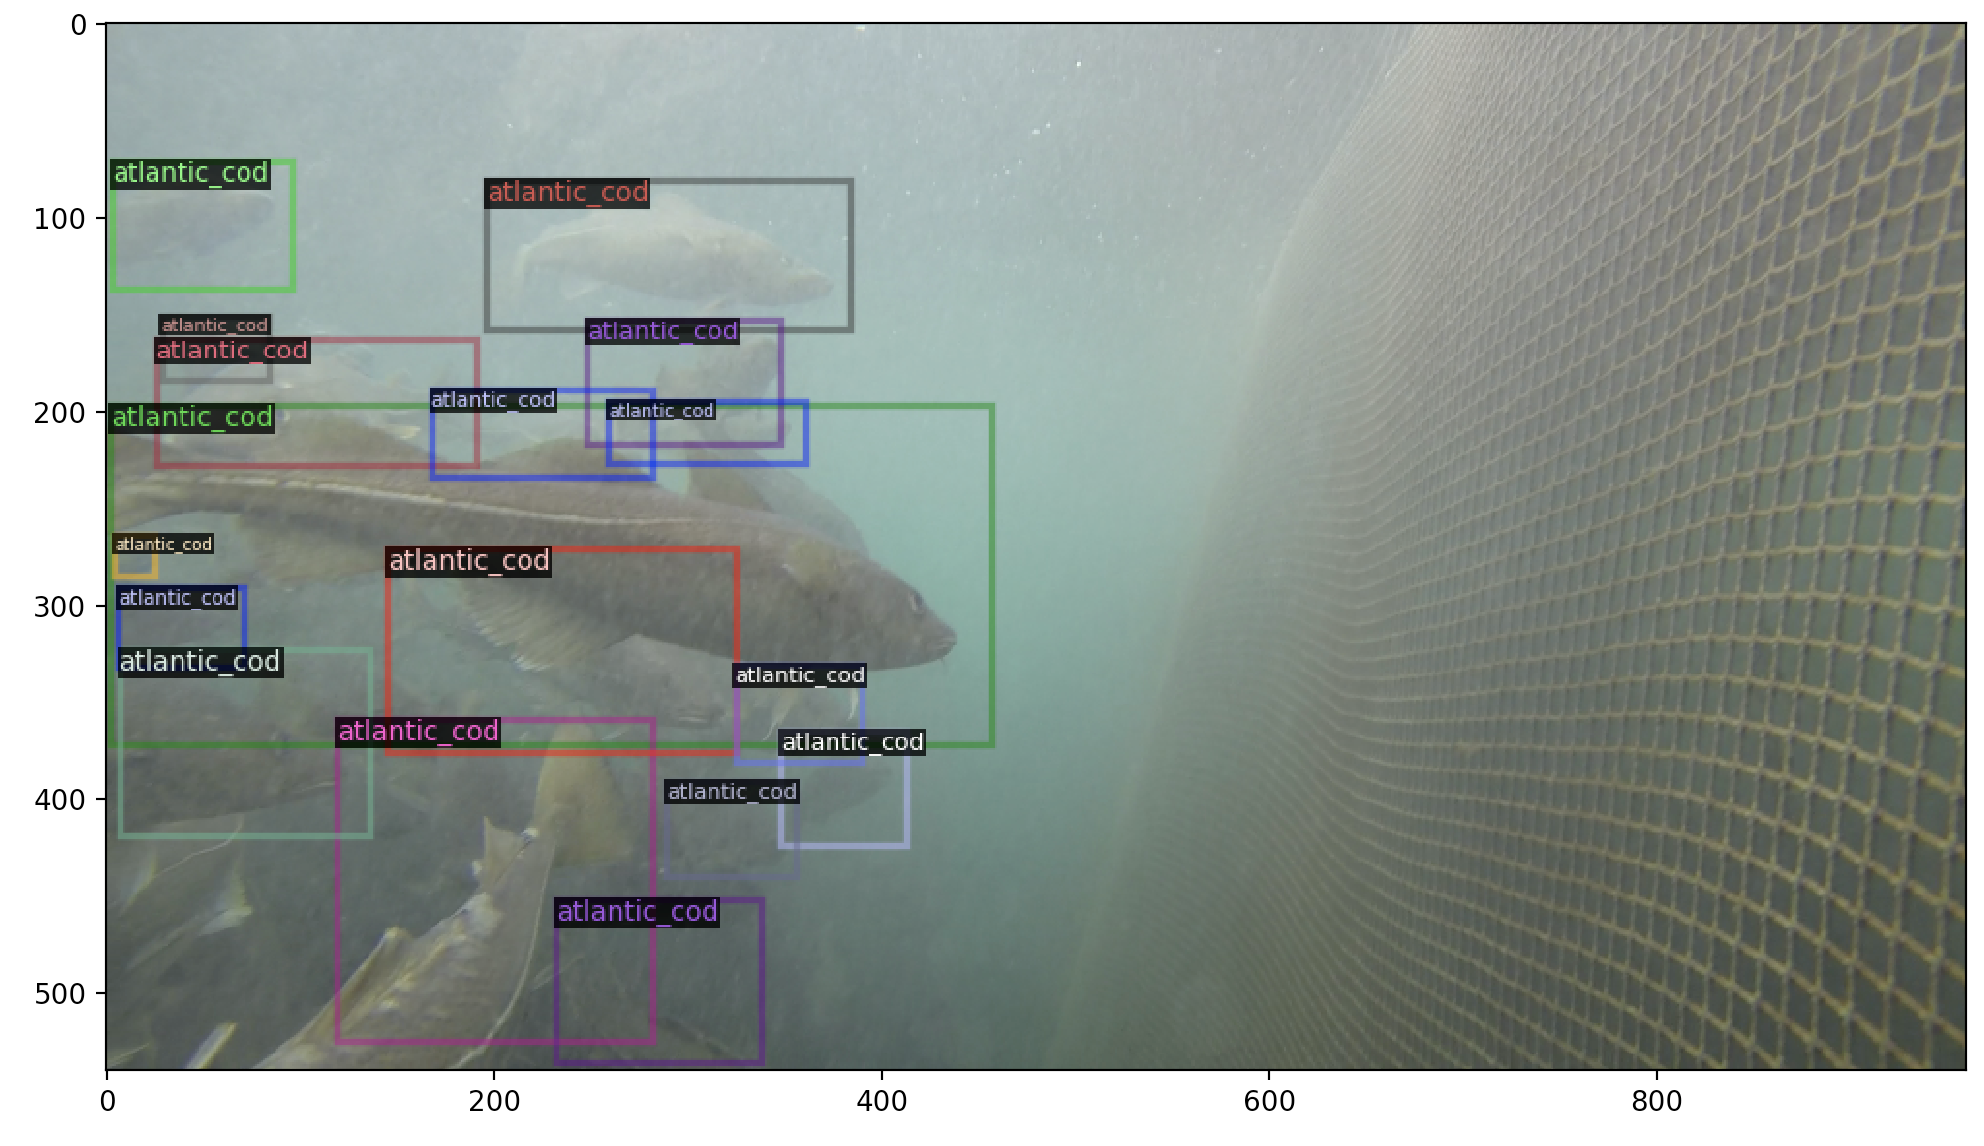
\includegraphics[scale=0.35]{figures/retinanet_cod}
\caption{\small \sl Figuren viser objektdeteksjon av torsk i lagringsmerd med RetinaNet. \label{fig:retinenet_inference}} 
\end{center} 
\end{figure} 

Ettersom OpenCV kunne ikke laste inn en PyTorch modell da denne oppgaven ble skrevet, så ble inferens gjort med Python, og det ble ikke gjort et forsøk på å gjøre inference i sanntid på en videostrøm med RetinaNet. Se resultater i figur \ref{fig:retinenet_inference} og \ref{fig:inference}.

Koden for inferens er under.

\begin{lstlisting}[language=Python, caption=Inferens RetinaNet i inference.py]
def video_read_write(video_path):
    """
    Read video frames one-by-one, flip it, and write in the other video.
    video_path (str): path/to/video
    """
    video = cv2.VideoCapture(video_path)
    
    # Check if camera opened successfully
    if not video.isOpened(): 
        print("Error opening video file")
        return
    
    # create video writer
    width = int(video.get(cv2.CAP_PROP_FRAME_WIDTH))
    height = int(video.get(cv2.CAP_PROP_FRAME_HEIGHT))
    frames_per_second = video.get(cv2.CAP_PROP_FPS)
    num_frames = int(video.get(cv2.CAP_PROP_FRAME_COUNT))
    
    isStreamOpen = False
    while video.isOpened():
        ret, frame = video.read()
        
        if ret:
            outputs = predictor(frame)

            #print(outputs)
            v = Visualizer(frame[:, :, ::-1],
                           metadata=test_metadata, 
                           scale=0.8
            )

            instances = outputs["instances"].to("cpu")

            v = v.draw_instance_predictions(instances)

            plt.imsave('outputs/frame_intermediate.png', v.get_image())

            if isStreamOpen == False:
                img = cv2.imread('outputs/frame_intermediate.png')
                height, width, layers = img.shape
                size = (width,height)
                out = cv2.VideoWriter('out.avi',cv2.VideoWriter_fourcc(*'DIVX'),
                		      frames_per_second, size)
                isStreamOpen = True

            img = cv2.imread('outputs/frame_intermediate.png')

            cv2.putText(img, 'num instances: ' + str(len(instances)), (5,100),
            		cv2.FONT_HERSHEY_SIMPLEX, 3, (0, 255, 0), 2, cv2.LINE_AA)
            out.write(img)

            print ('num instances: ' + str(len(instances)))
        else:
            break
    
    out.release()
    video.release()
    
    return

cfg.DATASETS.TEST = (test_data_name,)

# create a predictor instance with the configuration (it has our fine-tuned model)
# this predictor does prdiction on a single image
predictor = DefaultPredictor(cfg)

# create directory for evaluation
eval_dir = os.path.join(cfg.OUTPUT_DIR, 'coco_eval')
os.makedirs(eval_dir, exist_ok=True)

# create evaluator instance with coco evaluator
evaluator = COCOEvaluator(dataset_name=test_data_name,
                          cfg=cfg,
                          distributed=False,
                          output_dir=eval_dir)

# create validation data loader
val_loader = build_detection_test_loader(cfg, test_data_name)

# start validation 
inference_on_dataset(trainer.model, val_loader, evaluator)

# Run inference on video
video_read_write('in.mp4')
\end{lstlisting}

\subsubsection{OpenCV program} \label{part:opencv}

OpenCV (Open Source Computer Vision Library) er en åpenkildekode maskinsyn og maskinlæring programvarebibliotek. OpenCV ble laget for å levere en kjent infrastruktur for maskinsynprogrammer, OpenCV teamet ønsker å gjøre maskinsensorikk mer utbredt i kommersielle produkter. OpenCV er et produkt gitt ut under BSD-lisensen, det gjør biblioteket tilgjengelig for bedrifter som ønsker å anvende kildekoden. \cite{OpenCV Team 2020}

OpenCV har C++, Python, Java og MATLAB grensesnitt og støtter Windows, Linux, Android og macOS. OpenCV Teamet forsøker først og fremst å levere sanntids maskinsyn for dataprogrammer og drar nytte av prosessorteknologi slik som MMX og SSE instruksjoner når de er tilgjengelige. CUDA og OpenCL støtte var under utvikling, men var enda ikke tilgjengelig da denne oppgaven ble skrevet. Det hadde gjort dataprogrammet mye raskere, den ville dratt nytte av GPU-en og ikke bare CPU-en på maskinen. OpenCV er skrevet i C++ og virker uten konflikter med STL datastrukturer. \cite{OpenCV Team 2020}

Det ble skrevet et C++ program som bruker OpenCV til sanntids fiskedeteksjon med YOLOv4 modellen. OpenCV hadde fortsatt dårlig støtte av ONIX formatet, caffe2 formatet, og PyTorch da denne oppgaven ble skrevet. OpenCV 3.4 ble anvendt, da den fikk nylig støtte for YOLOv4. \cite{Batanina 2020}

\begin{figure}
\begin{center} 
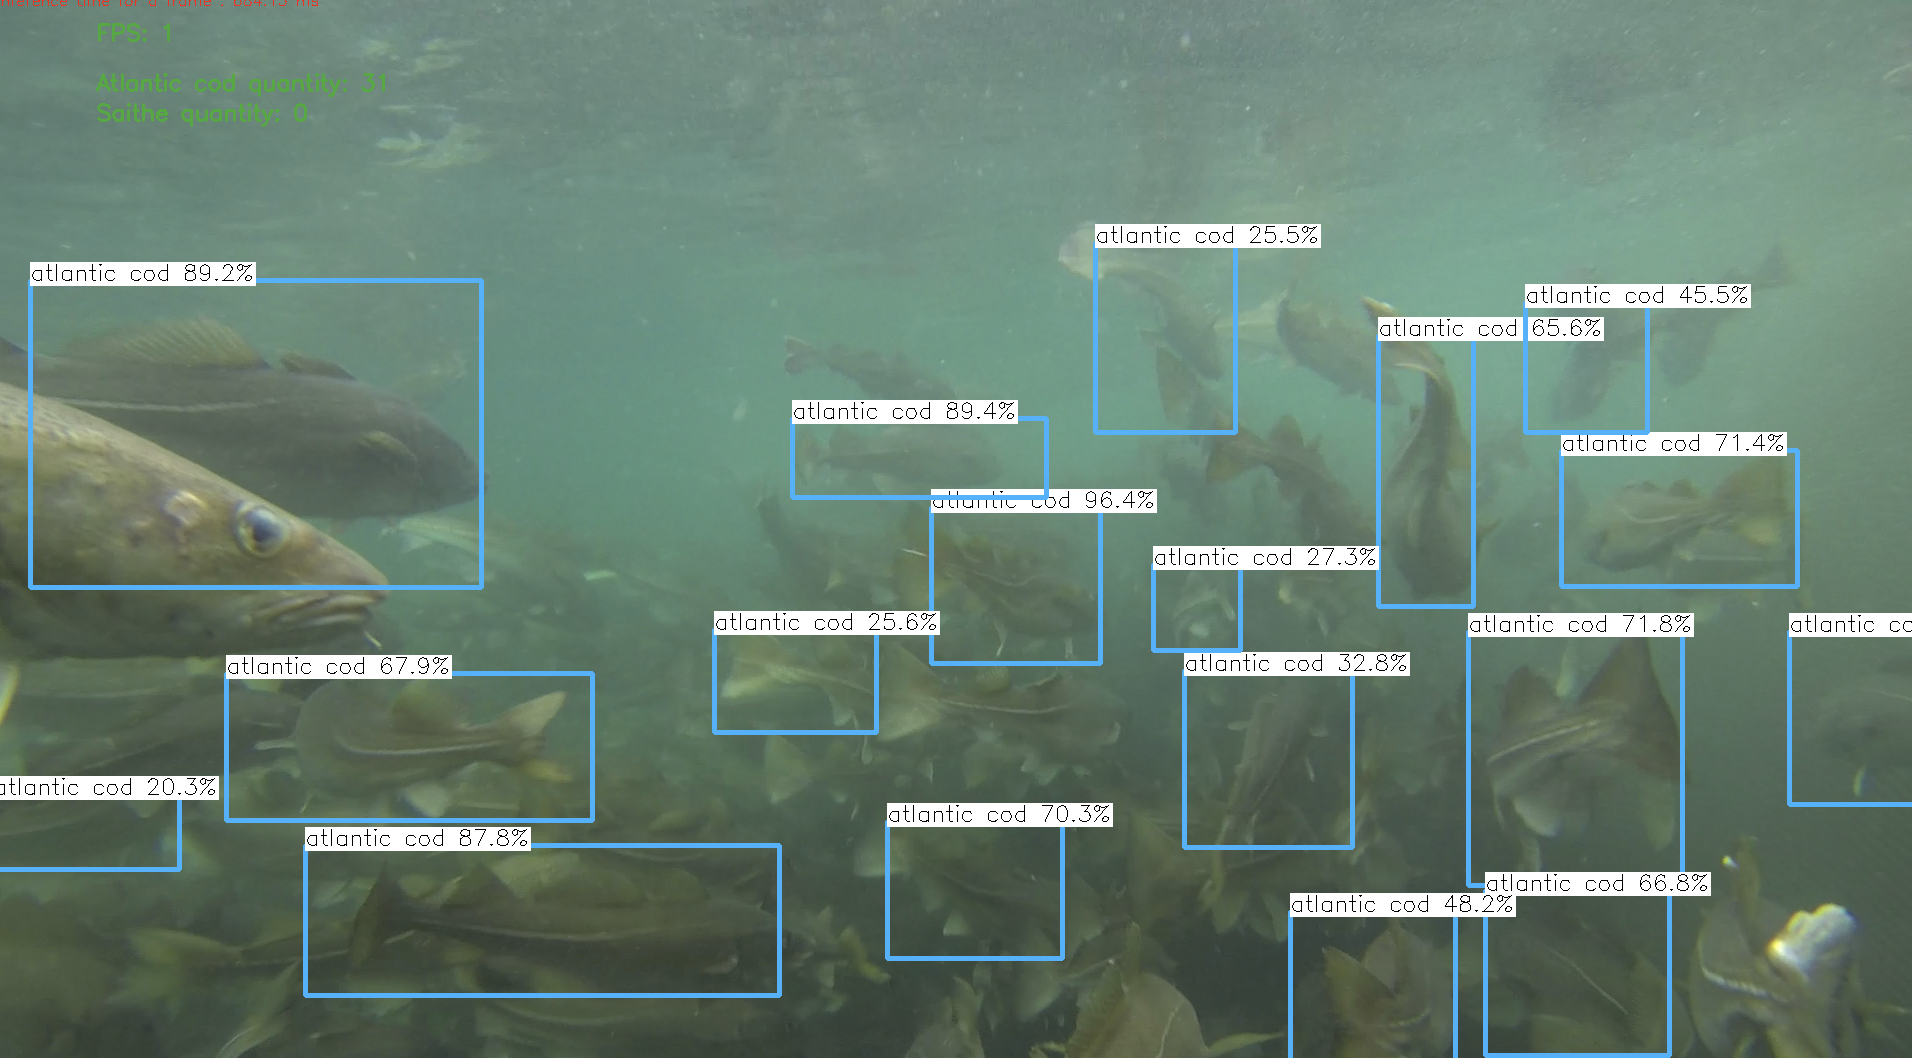
\includegraphics[scale=0.35]{figures/inference_yolo}
\caption{\small \sl Figuren viser inferens med YOLOv4. Rundt fiskene så lager YOLOv4 bounding boxes der den tror det finnes fisk, og gir den en label basert på det den tror at det er. Her får alle fiskene labelen ``atlantic cod'', dette er fra en lagringsmerd med torsk. Ved siden av navnet av klassen så står det hvor sikker nettverket er på at den har funnet en torsk, presisjonen av inferensen. I grønn tekst, øverst til venstre, står det at algoritmen kan telle 31 torsk i bildet, og 0 sei. \label{fig:yolo_inference}} 
\end{center} 
\end{figure} 

Inferens med YOLOv4 ble gjort i OpenCV programmet. Programmet heter OBJECT\_DETECTOR, den laster inn en YOLOv4 konfigurasjon, en modell, og en videostrøm. Videostrømmen kan komme fra et kamera koblet til maskinen eller en fil på filsystemet. Programmet analyserer videostrømmen og logger mengden torsk og sei som blir observert. Se figur \ref{fig:yolo_inference}.

Når en lager et C++ program så må en kompilator og build-system bli valgt. For Windows så ble msvc++, som er en del av Visual Studio Community 2019, valgt. På macOS så ble clang brukt. Build-systemet cmake ble valgt. Alle disse verktøyene er tilgjengelig gratis, msvc++ er det eneste verktøyet som ikke er et åpen kildekodeprosjekt i tillegg til å være gratis. CMakeLists.txt beskriver C++ programmet. CMakelists.txt er en konfigurasjonsfil for cmake build-systemet, et av build systemene som kan brukes til å holde styr på C++ programmer. Det er nyttig å ha et IDE, en Intergrated Development Environment, når man programmerer i C++. QtCreator open source er et velutviklet IDE som kan laste inn cmake prosjekter.

OpenCV-prosjektet bruker også cmake, og er også skrevet i C++. Her installeres OpenCV fra kommandolinjen på et unix system.

\begin{verbatim}
mkdir opencv-3.4
cd opencv-3.4
git clone https://github.com/opencv/opencv
git clone https://github.com/opencv/opencv_contrib
cd opencv_contrib
git checkout 3.4
cd modules
dir=$(pwd)
cd ../../opencv
git checkout 3.4
mkdir build
cd build
cmake OPENCV_EXTRA_MODULES_PATH=$dir ..
make
make install
\end{verbatim}

\begin{figure}
\begin{center} 
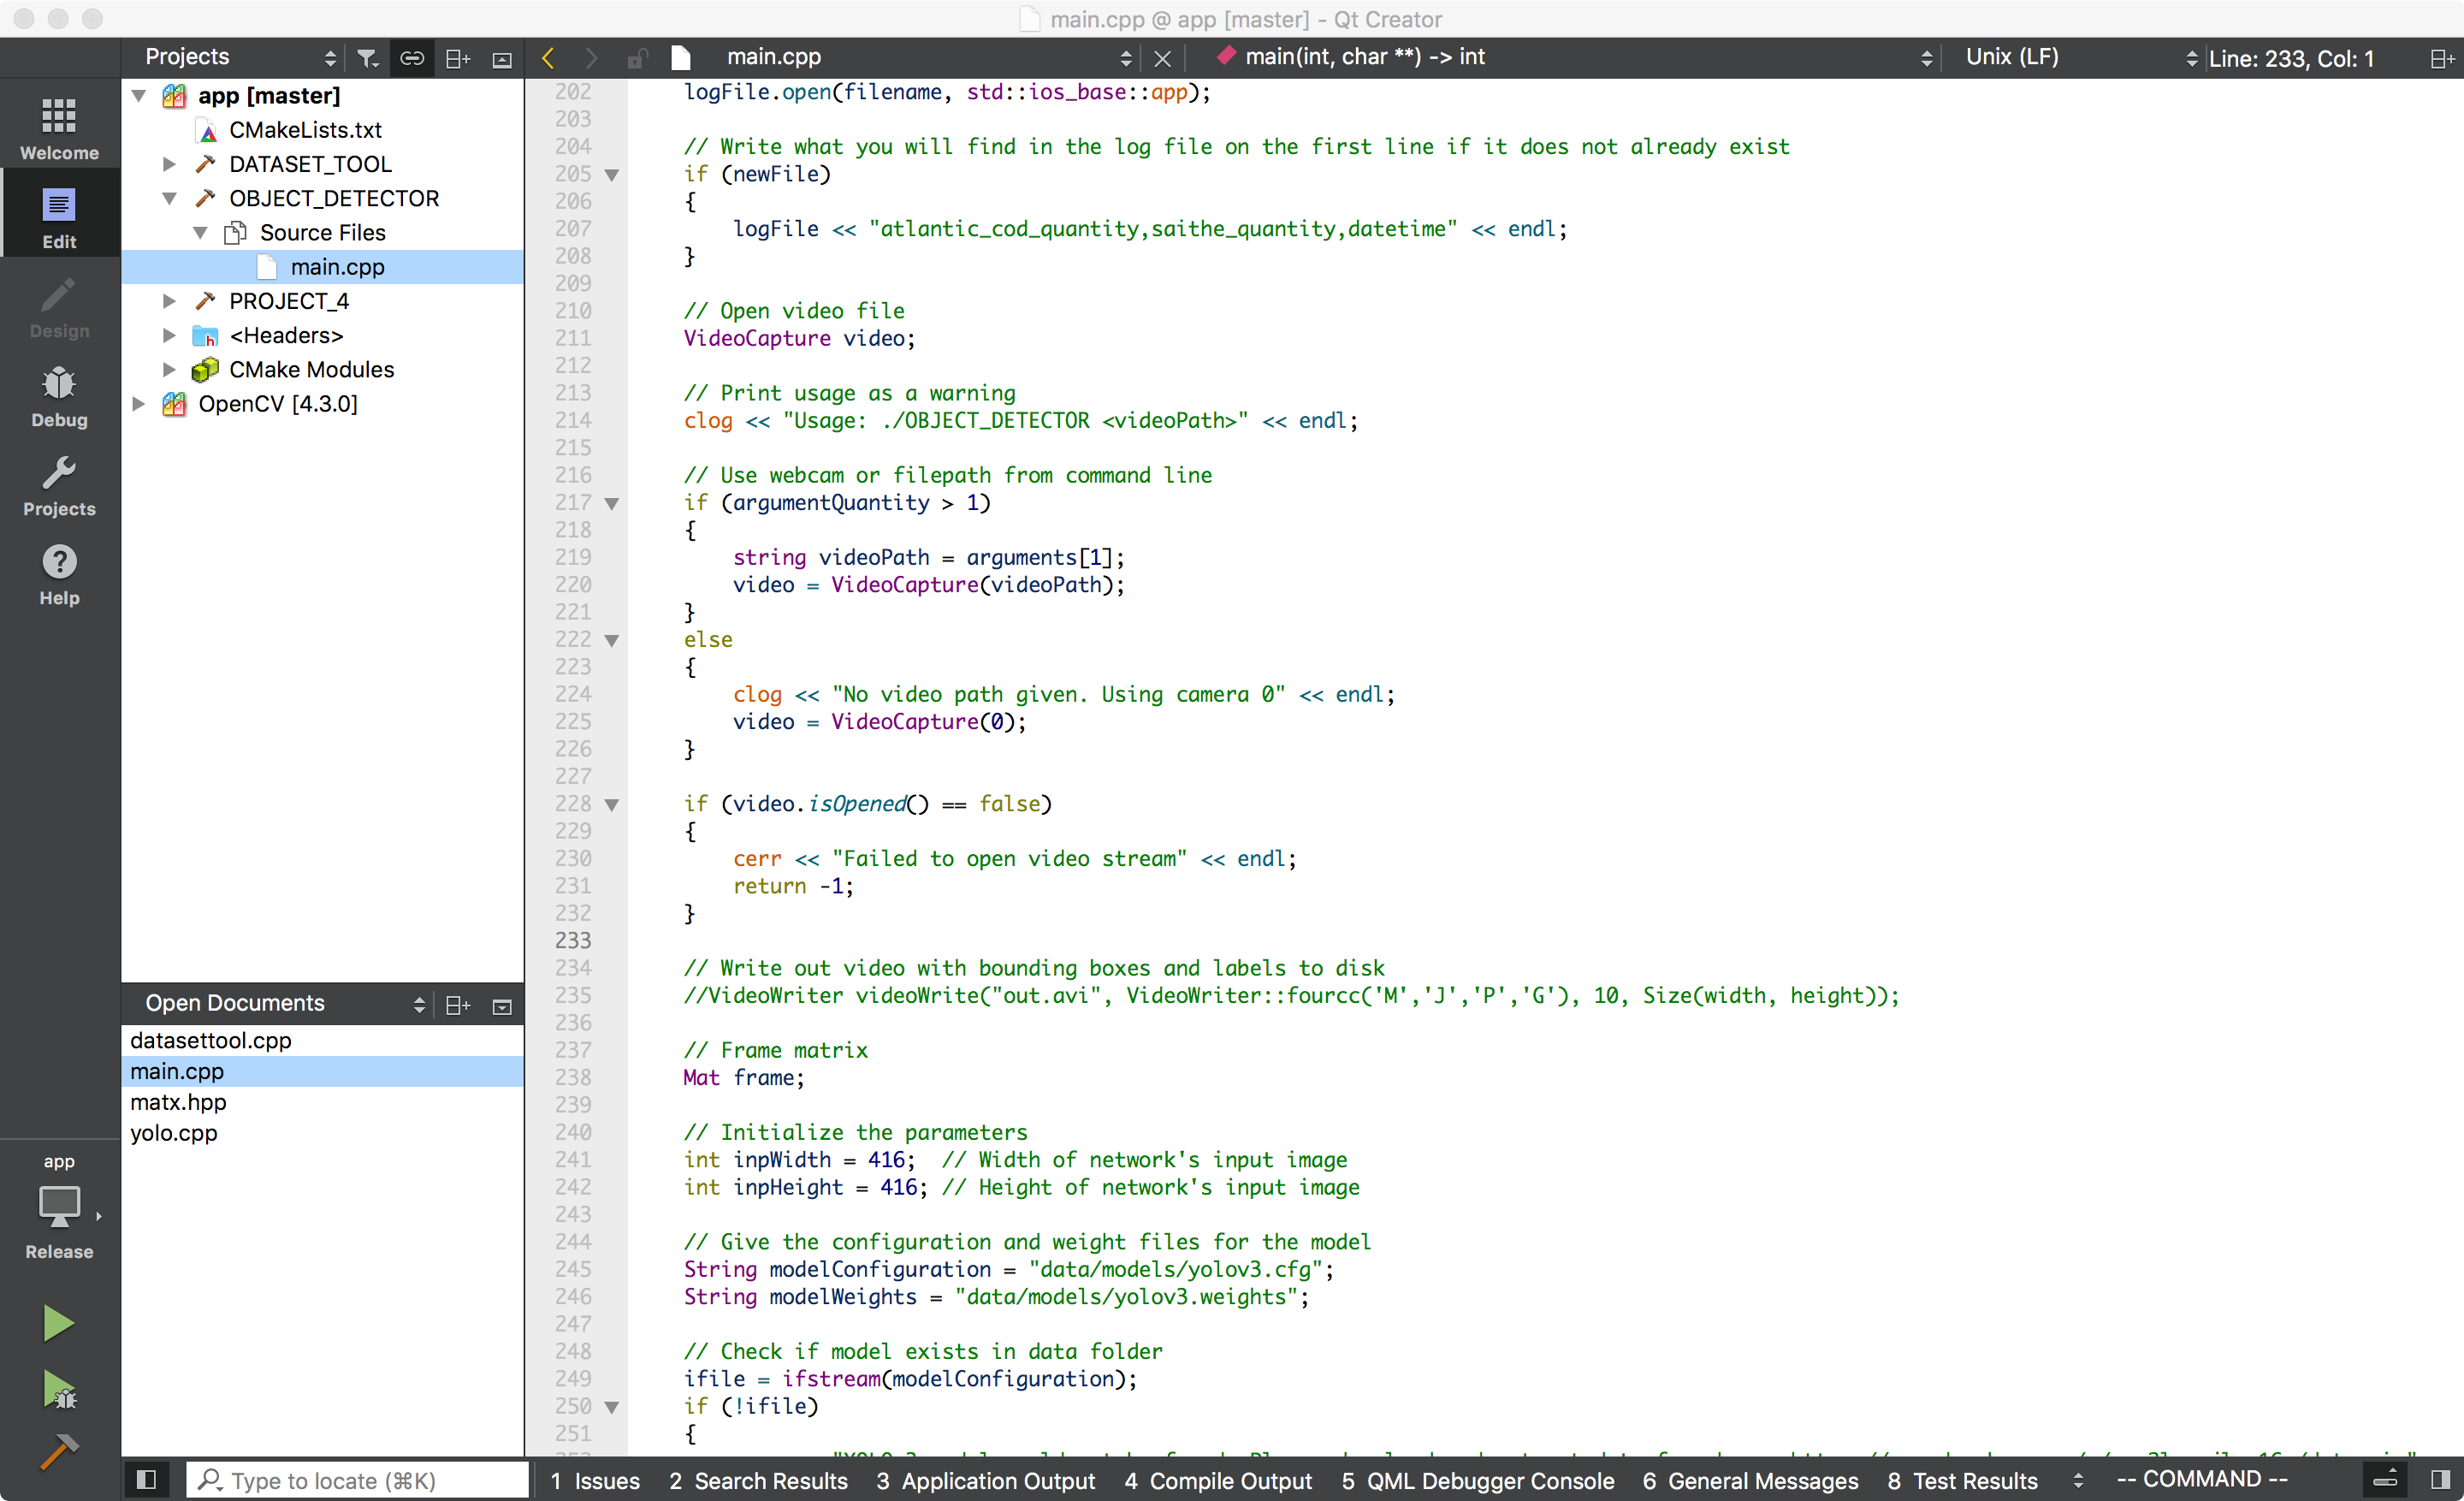
\includegraphics[scale=0.2]{figures/qtcreator}
\caption{\small \sl QtCreator. \label{fig:qtcreator}} 
\end{center} 
\end{figure} 

Det er også mulig å kompilere OpenCV med hjelp fra QtCreator. QtCreator open source ble lastet ned fra \url{https://www.qt.io/download}. CMakeLists.txt i opencv-3.4/opencv ble åpnet i QtCreator. OPENCV\_EXTRA\_MODULES\_PATH ble satt til opencv\_contrib/modules på filsystemet. Dette kan gjøres fra Projects modusen i QtCreator. Se sidepanelet i figur \ref{fig:qtcreator}.

Anaconda individual edition med python 2 ble brukt. Det ble laget en cmake CMakeLists.txt fil for prosjektet. Denne burde muligens endres om andre ønsker å kompilere prosjektet, merk at anaconda ble installert til hjemmemappen til brukeren. Prosjektet består av to programmer. OBJECT\_DETECTOR gjør fiskedeteksjon. Se figur \ref{fig:yolo_inference}. DATASET\_TOOL ble brukt til å lage label data ut av videoer. Se figur \ref{fig:dataset_tool}.

\begin{lstlisting}[language=, caption=CMakeLists.txt]
cmake_minimum_required(VERSION 2.8.12)

PROJECT(app)
SET(CMAKE_CXX_STANDARD 14)

SET(Python2_ROOT_DIR ${PYTHONHOME})

find_package(Python2 COMPONENTS Development NumPy)

SET(OpenCV_DIR C:/opencv-3.4/opencv/build)

if( UNIX )
    include_directories(~/anaconda2/include/python2.7 ~/anaconda2/lib/python2.7/\
    site-packages/numpy/core/include/ ~/anaconda2/include)
else()
    include_directories(${PYTHON_INCLUDE_DIRS} ~/Anaconda2/Lib/site-packages/numpy/core/\
    	include)
endif()

if(MSVC)
SET(CMAKE_CXX_FLAGS_RELEASE "${CMAKE_CXX_FLAGS_RELEASE} /MT")
endif()

find_package( OpenCV REQUIRED )

set(OpenCV_STATIC ON) # Easier to share binaries

include_directories( ${OpenCV_INCLUDE_DIRS} )

# If the package has been found, several variables will
# be set, you can find the full list with descriptions
# in the OpenCVConfig.cmake file.
# Print some message showing some of them
message(STATUS "OpenCV library status:")
message(STATUS "    config: ${OpenCV_DIR}")
message(STATUS "    version: ${OpenCV_VERSION}")
message(STATUS "    libraries: ${OpenCV_LIBS}")
message(STATUS "    include path: ${OpenCV_INCLUDE_DIRS}")

add_executable(OBJECT_DETECTOR main.cpp)
target_include_directories(OBJECT_DETECTOR PRIVATE ${PYTHON2_INCLUDE_DIRS} \
	${PYTHON2_NUMPY_INCLUDE_DIRS})
target_link_libraries(OBJECT_DETECTOR PRIVATE ${OpenCV_LIBS} Python2::Python )

add_executable(DATASET_TOOL datasettool.cpp)
target_include_directories(DATASET_TOOL PRIVATE ${PYTHON2_INCLUDE_DIRS}\
	 ${PYTHON2_NUMPY_INCLUDE_DIRS})
target_link_libraries(DATASET_TOOL PRIVATE ${OpenCV_LIBS} Python2::Python )
\end{lstlisting}

main.cpp er kildekoden til OBJECT\_DETECTOR. Først lastes bibliotekene inn.

\begin{lstlisting}[language=C++, caption=main.cpp]
#include <opencv2/opencv.hpp>
#include <opencv2/dnn.hpp>
//#include <opencv2/tracking.hpp>
#include <fstream>
//#include "matplotlibcpp.h"
#include <chrono>
#include <ctime>

using namespace std;
//using namespace matplotlibcpp;
using namespace cv::dnn;
using namespace cv;

// globals
float objectnessThreshold; // Objectness threshold
float confThreshold; // Confidence threshold
float nmsThreshold;  // Non-maximum suppression threshold
int inpWidth;  // Width of network's input image
int inpHeight; // Height of network's input image
vector<string> classes;

vector<Rect2d> bboxes;
int codQuantity, saitheQuantity;

string objectLabel;

const char *WINDOW_TITLE = "Press ESC to quit";
\end{lstlisting}

getOutputsNames henter ut label navn fra det ytterste laget i modellen. Se figur \ref{fig:deep}.

\begin{lstlisting}[language=C++, caption=main.cpp]
// Get the names of the output layers
auto getOutputsNames(const Net& net)
{
    static vector<String> names;
    if (names.empty())
    {
        // Get the indices of the output layers, i.e. the layers with unconnected outputs
        vector<int> outLayers = net.getUnconnectedOutLayers();

        // Get the names of all the layers in the network
        vector<String> layersNames = net.getLayerNames();

        // Get the names of the output layers in names
        names.resize(outLayers.size());
        for (size_t i = 0; i < outLayers.size(); ++i)
            names[i] = layersNames[outLayers[i] - 1];
    }
    return names;
}
\end{lstlisting}

drawPred lager en bounding box rundt objektene som detekteres av modellen.

\begin{lstlisting}[language=C++, caption=main.cpp]
// Draw the predicted bounding box
void drawPred(int classId, float conf, int left, int top, int right, int bottom, Mat& frame)
{
    // Draw a rectangle displaying the bounding box
    rectangle(frame, Point(left, top), Point(right, bottom), Scalar(255, 178, 50), 3);

    // Get the label for the class name and its confidence
    string label = format("%.1f", conf * 100);
    if (!classes.empty())
    {
        CV_Assert(classId < (int)classes.size());
        label = classes[classId] + " " + label + "\%";
    }

    // Display the label at the top of the bounding box
    int baseLine;
    Size labelSize = getTextSize(label, FONT_HERSHEY_SIMPLEX, 0.5, 1, &baseLine);
    top = max(top, labelSize.height);
    rectangle(frame,
    		   Point(left, top - round(1.5*labelSize.height)),
		   Point(left + round(1.5*labelSize.width),
		   top + baseLine),
		   Scalar(255, 255, 255),
		   FILLED);
    putText(frame, label, Point(left, top), FONT_HERSHEY_SIMPLEX, 0.75, Scalar(0,0,0),1);

    objectLabel = label;
}
\end{lstlisting}

postprocess henter alle instanser av fiskene i et bilde som er over en non-maxima suppression confidence boundary. Deretter sjekker den om objektet er en torsk eller sei, og teller mengden torsk og sei i bildet.

\begin{lstlisting}[language=C++, caption=main.cpp]
// Remove the bounding boxes with low confidence using non-maxima suppression
void postprocess(Mat& frame, const vector<Mat>& outs)
{
    vector<int> classIds;
    vector<float> confidences;
    vector<Rect> boxes;

    codQuantity = 0;
    saitheQuantity = 0;

    for (size_t i = 0; i < outs.size(); ++i)
    {
        // Scan through all the bounding boxes output from the network and keep only the
        // ones with high confidence scores. Assign the box's class label as the class
        // with the highest score for the box.
        float* data = (float*)outs[i].data;
        for (int j = 0; j < outs[i].rows; ++j, data += outs[i].cols)
        {
            Mat scores = outs[i].row(j).colRange(5, outs[i].cols);
            Point classIdPoint;
            double confidence;
            // Get the value and location of the maximum score
            minMaxLoc(scores, 0, &confidence, 0, &classIdPoint);

            if (confidence > confThreshold)
            {
                if (classes[classIdPoint.x] == "atlantic cod") {
                    codQuantity++;
                }
                else if (classes[classIdPoint.x] == "saithe")
                {
                    saitheQuantity++;
                }

                int centerX = (int)(data[0] * frame.cols);
                int centerY = (int)(data[1] * frame.rows);
                int width = (int)(data[2] * frame.cols);
                int height = (int)(data[3] * frame.rows);
                int left = centerX - width / 2;
                int top = centerY - height / 2;

                classIds.push_back(classIdPoint.x);
                confidences.push_back((float)confidence);
                boxes.push_back(Rect(left, top, width, height));
            }
        }
    }

    // Perform non maximum suppression to eliminate redundant overlapping boxes with
    // lower confidences
    vector<int> indices;
    NMSBoxes(boxes, confidences, confThreshold, nmsThreshold, indices);
    for (size_t i = 0; i < indices.size(); ++i)
    {
        int idx = indices[i];
        Rect box = boxes[idx];
        drawPred(classIds[idx], confidences[idx], box.x, box.y,
                 box.x + box.width, box.y + box.height, frame);
    }
}
\end{lstlisting}

main er programmets entry point. Det er her dataprogrammet starter. Den åpner en logg, log.csv, og så åpner den en videostrøm. Deretter laster den inn YOLOv4 modellen.

\begin{lstlisting}[language=C++, caption=main.cpp]
int main(int argumentQuantity, char *arguments[])
{
    // Configuration for log file
    string filename = "log.csv";
    bool newFile = true;

    // Check if log file exists
    ifstream ifile(filename);
    if (ifile)
    {
        newFile = false;
    }

    // Open log file
    ofstream logFile;
    logFile.open(filename, std::ios_base::app);

    // Write what you will find in the log file on the first line
    // if it does not already exist
    if (newFile)
    {
        logFile << "atlantic_cod_quantity,saithe_quantity,datetime" << endl;
    }

    // Open video file
    VideoCapture video;

    // Print usage as a warning
    clog << "Usage: ./OBJECT_DETECTOR <videoPath>" << endl;

    // Use webcam or filepath from command line
    if (argumentQuantity > 1)
    {
        string videoPath = arguments[1];
        video = VideoCapture(videoPath);
    }
    else
    {
        clog << "No video path given. Using camera 0" << endl;
        video = VideoCapture(0);
    }

    if (video.isOpened() == false)
    {
        cerr << "Failed to open video stream" << endl;
        return -1;
    }

    // Frame matrix
    Mat frame;

    // Initialize the parameters
    int inpWidth = 416;  // Width of network's input image
    int inpHeight = 416; // Height of network's input image

    // Give the configuration and weight files for the model
    String modelConfiguration = "data/models/yolov-obj.cfg";
    String modelWeights = "data/models/yolo.weights";

    // Check if model exists in data folder
    ifile = ifstream(modelConfiguration);
    if (!ifile)
    {
        cerr << "YOLOv4 model could not be found." << endl;
        return -1;
    }

    // Load the network
    Net net = readNetFromDarknet(modelConfiguration, modelWeights);

    // Load names of classes
    string classesFile = "data/models/obj.names";
    ifstream ifs(classesFile.c_str());
    string line;
    while (getline(ifs, line)) classes.push_back(line);

    // Configure user interface
    namedWindow(WINDOW_TITLE, WINDOW_AUTOSIZE);
\end{lstlisting}

Den neste kodesnutten er programmets main loop. Denne koden repeteres til videoen har gått tomt for bilder, eller at brukeren trykker på ESC på tastaturet. For hvert bilde i videostrømmen så lagres antall torsk og sei observert til log.csv, med mindre det er ingen torsk eller sei som blir oppdaget.

\begin{lstlisting}[language=C++, caption=main.cpp]
    // Main loop
    bool isAlive = true;
    const int ESCAPE_KEYCODE = 27;
    const int DELAY_MILLISECONDS = 1;

    int key;

    while(isAlive)
    {
        key = waitKey(DELAY_MILLISECONDS);

        if (key == ESCAPE_KEYCODE)
        {
            isAlive = false;
            break;
        }

        double timer = (double)getTickCount();

        video >> frame;

        if (frame.empty())
        {
            isAlive = false;
            break;
        }

        // Create a 4D blob from a frame.
        Mat blob;
        blobFromImage(frame, 
        		blob,
        		1/255.0,
        		Size(inpWidth, inpHeight),
        		Scalar(0,0,0),
        		true,
        		false);

        //Sets the input to the network
        net.setInput(blob);

        // Runs the forward pass to get output of the output layers
        vector<Mat> outs;
        net.forward(outs, getOutputsNames(net));

        // Remove the bounding boxes with low confidence
        postprocess(frame, outs);

        // Put efficiency information.
        // The function getPerfProfile returns the overall time for inference(t)
        // and the timings for each of the layers(in layersTimes)
        vector<double> layersTimes;
        double freq = getTickFrequency() / 1000;
        double t = net.getPerfProfile(layersTimes) / freq;
        string label = format("Inference time for a frame : %.2f ms", t);
        putText(frame, label, Point(0, 15), FONT_HERSHEY_SIMPLEX, 0.5, Scalar(0, 0, 255));

        float fps = getTickFrequency() / ((double)getTickCount() - timer);

        putText(frame,
        		    "FPS: " + std::to_string(int(fps)),
		    Point(100,50),
		    FONT_HERSHEY_SIMPLEX, 0.75,
		    Scalar(50,170,50), 2);
        putText(frame,
        		    "Atlantic cod quantity: " + std::to_string(codQuantity),
		    Point(100,100),
		    FONT_HERSHEY_SIMPLEX,
		    0.75,
		    Scalar(50,170,50),
		    2);
        putText(frame,
        		    "Saithe quantity: " + std::to_string(saitheQuantity),
		    Point(100,130),
		    FONT_HERSHEY_SIMPLEX,
		    0.75,
		    Scalar(50,170,50),
		    2);

        //videoWrite.write(frame);
        imshow(WINDOW_TITLE, frame);

        // Get the time
        auto end = std::chrono::system_clock::now();
        std::time_t end_time = std::chrono::system_clock::to_time_t(end);

        // Remove the newline after time which is typically included from the C library call
        char *time = ctime(&end_time);
        if (time[strlen(time)-1] == '\n') time[strlen(time)-1] = '\0';

        // Log cod and saithe quantities to csv file
        if (codQuantity > 0 || saitheQuantity > 0)
        {
            logFile << codQuantity << "," << saitheQuantity << ",\"" << time << "\"" << endl;
            cout << codQuantity << "," << saitheQuantity << ",\"" << time << "\"" << endl;
        }
    }

    logFile.close();

    video.release();
    //videoWrite.release();

    destroyAllWindows();

    return 0;
}
\end{lstlisting}

%\subsection{COCO Detection Evaluation} % For analyse kapittelet?

\subsection{Segmentering}

\begin{figure}[h!]
\begin{center} 
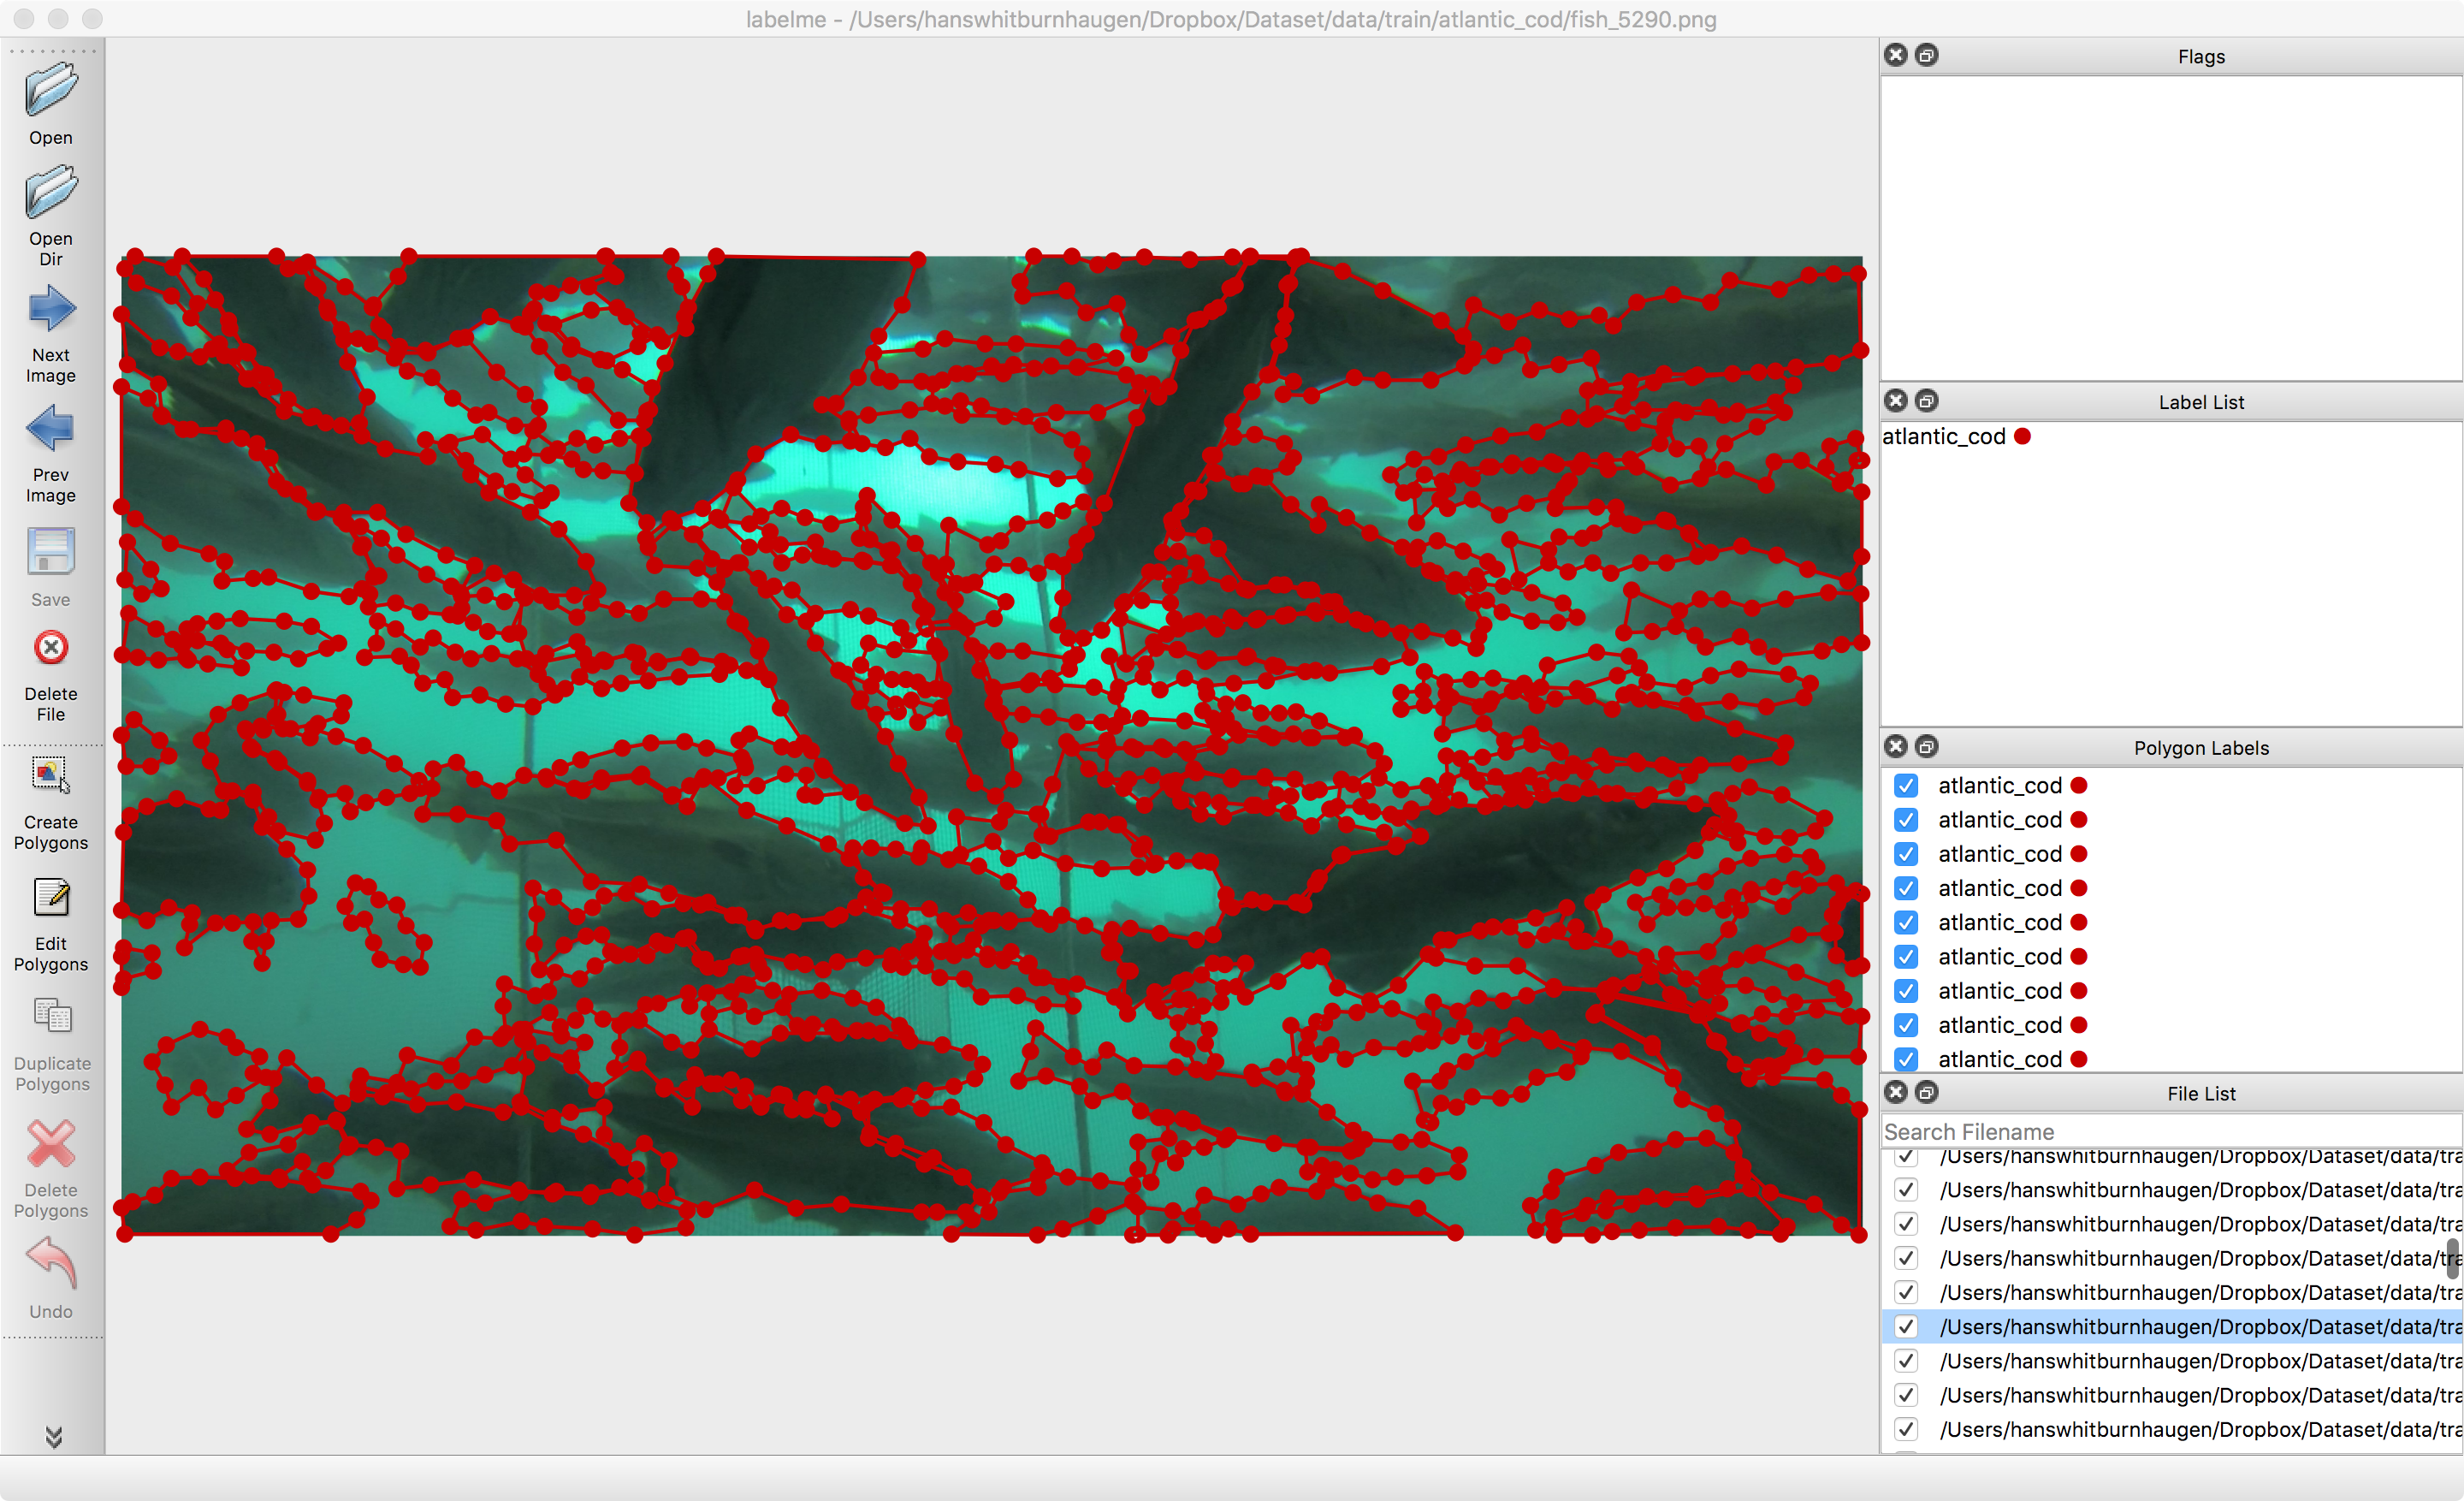
\includegraphics[scale=0.25]{figures/labelme}
\caption{\small \sl Figuren viser dataprogrammet labelme. \cite{Wada 2016} \label{fig:labelme}} 
\end{center} 
\end{figure} 
